\chapter{Introduction} \label{ch:intro}

Welcome to Dynare! \\

\section{About this Guide - approach and structure}
This User Guide \textbf{aims to help you master Dynare}'s main functionalities, from getting started to implementing advanced features. To do so, this Guide is structured around examples and offers practical advice. To root this understanding more deeply, though, this Guide also gives some background on Dynare's algorithms, methodologies and underlying theory. Thus, a secondary function of this Guide is to \textbf{serve as a basic primer} on DSGE model solving and Bayesian estimation. \\

This Guide will focus on the most common or useful features of the program, thus emphasizing \textbf{depth over breadth}. The idea is to get you to use 90\% of the program well and then tell you where else to look if you're interested in fine tuning or advanced customization.\\

This Guide is written mainly for an \textbf{advanced economist} - like a professor, graduate student or central banker - needing a powerful and flexible program to support and facilitate his or her research activities in a variety of fields. The sophisticated computer programmer, on the one hand, or the specialist of computational economics, on the other, may not find this Guide sufficiently detailed. \\

We recognize that the ``advanced economist'' may be either a beginning or intermediate user of Dynare. This Guide is written to accommodate both. If you're \textbf{new to Dynare}, we recommend starting with chapters \ref{ch:solbase} and \ref{ch:estbase}, which introduce the program's basic features to solve (including running impulse response functions) and estimate DSGE models, respectively. To do so, these chapters lead you through a complete hands-on example, which we recommend following from A to Z, in order to ``\textbf{learn by doing}''. Once you have read these two chapters, you will know the crux of Dynare's functionality and (hopefully!) feel comfortable using Dynare for your own work. At that point, though, you will probably find yourself coming back to the User Guide to skim over some of the content in the advanced chapters to iron out details and potential complications you may run into.\\

If you're instead an \textbf{intermediate user} of Dynare, you will most likely find the advanced chapters, \ref{ch:soladv} and \ref{ch:estadv}, more appropriate. These chapters cover more advanced features of Dynare and more complicated usage scenarios. The presumption is that you would skip around these chapters to focus on the topics most applicable to your needs and curiosity. Examples are therefore more concise and specific to each feature; these chapters read a bit more like a reference manual.\\

We also recognize that you probably have had repeated if not active exposure to programming and are likely to have a strong economic background. Thus, a black box solution to your needs is inadequate. To hopefully address this issue, the User Guide goes into some depth in covering the \textbf{theoretical underpinnings and methodologies that Dynare follows} to solve and estimate DSGE models. These are available in the ``behind the scenes of Dynare'' chapters \ref{ch:solbeh} and \ref{ch:estbeh}. These chapters can also serve as a \textbf{basic primer} if you are new to the practice of DSGE model solving and Bayesian estimation. \\

Finally, besides breaking up content into short chapters, we've introduced two different \textbf{markers} throughout the Guide to help streamline your reading.
\begin{itemize}
\item \textbf{\textsf{TIP!}} introduces advice to help you work more efficiently with Dynare or solve common problems.  
\item \textbf{\textsf{NOTE!}} is used to draw your attention to particularly important information you should keep in mind when using Dynare. 
\end{itemize} 


\section{What is Dynare?}
Before we dive into the thick of the ``trees'', let's have a look at the ``forest'' from the top \ldots just what is Dynare? \\

\textbf{Dynare is a powerful and highly customizable engine, with an intuitive front-end interface, to solve, simulate and estimate DSGE models}. \\

In slightly less flowery words, it is a pre-processor and a collection of Matlab routines that has the great advantages of reading DSGE model equations written almost as in an academic paper. This not only facilitates the inputting of a model, but also enables you to easily share your code as it is straightforward to read by anyone.\\
\begin{figure} \label{fig:dyn}
\begin{center} 
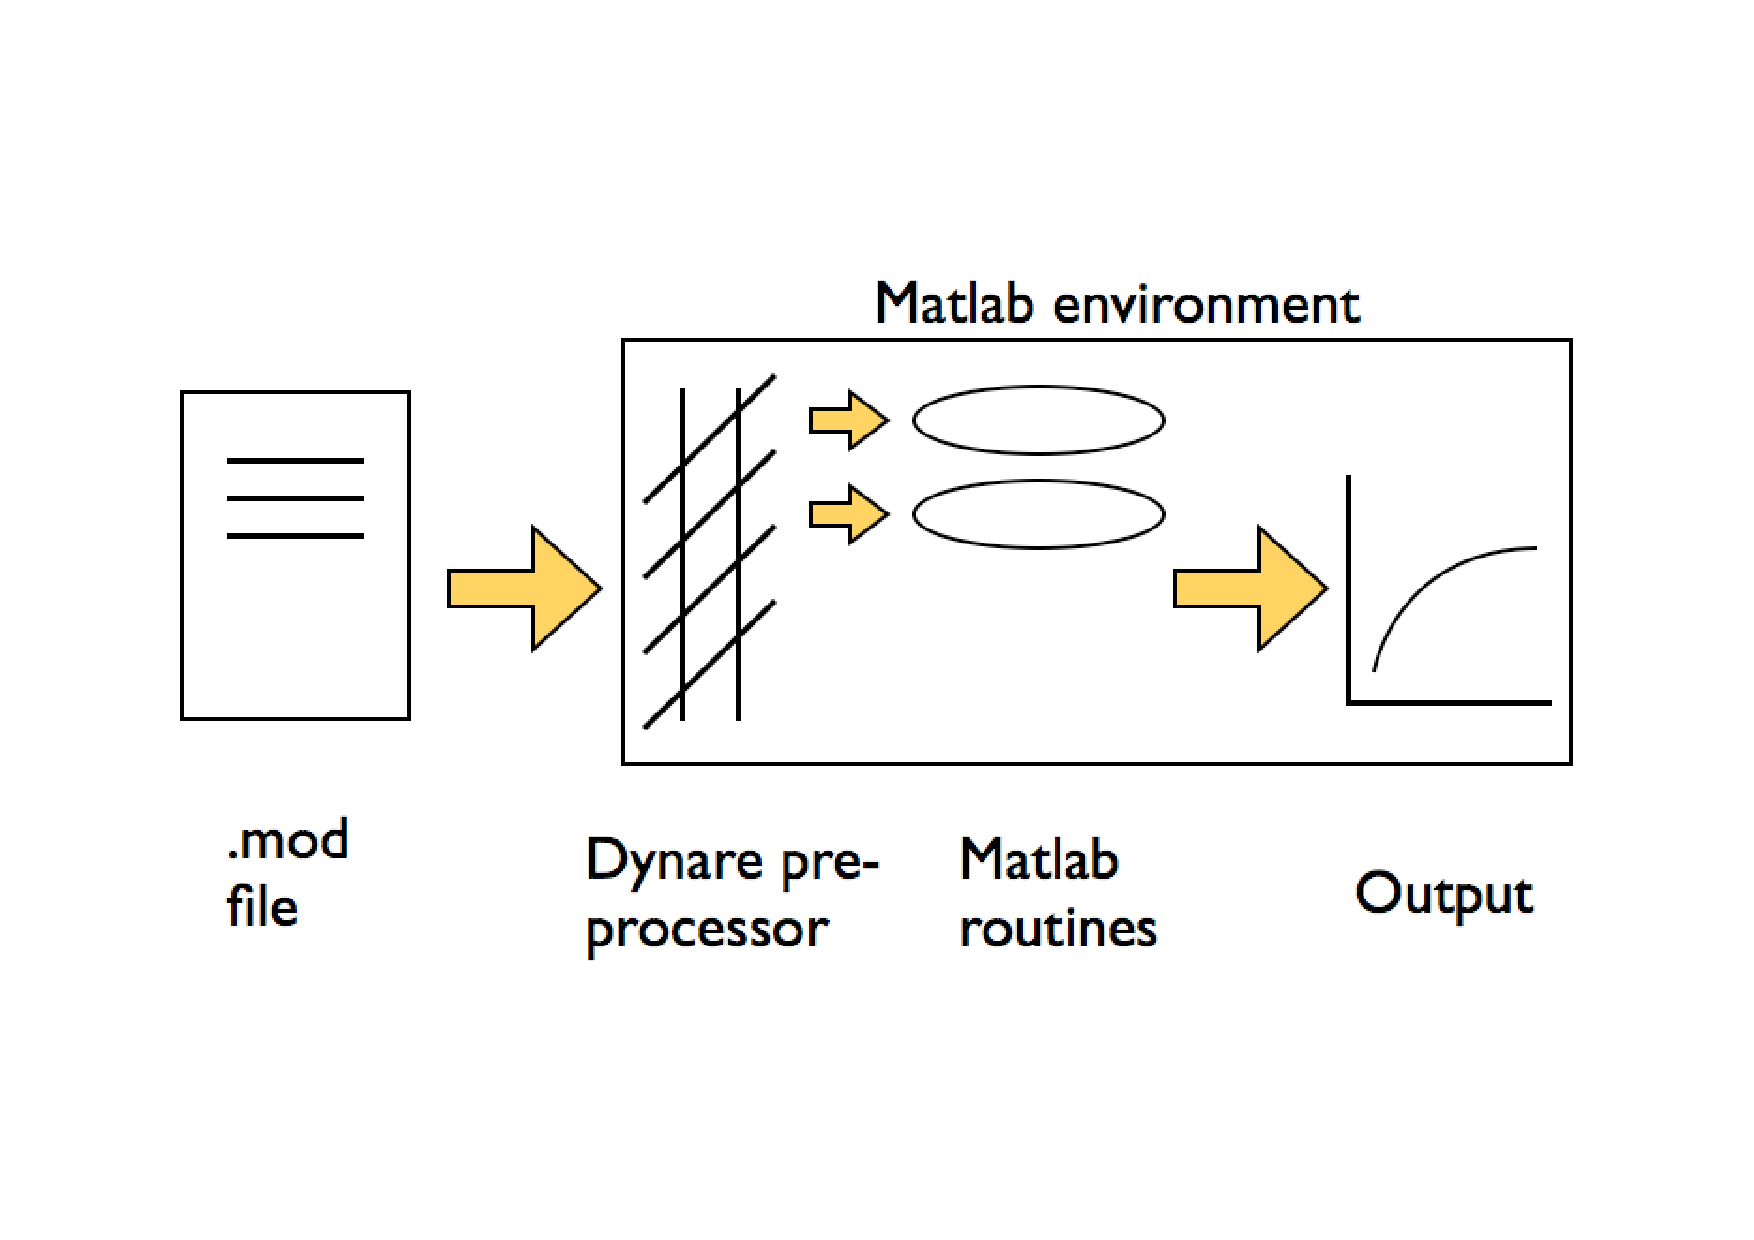
\includegraphics[width=1.0\textwidth]{P_DynareStruct2} 
\end{center} 
\caption[Dynare, a bird's eyeview]{The .mod file being read by the Dynare pre-processor, which then calls the relevant Matlab routines to carry out the desired operations and display the results.} 
\end{figure}

Figure \ref{fig:dyn} gives you an overview of the way Dynare works. Basically, the model and its related attributes, like a shock structure for instance, is written equation by equation in an editor of your choice. The resulting file will be called the .mod file. That file is then called from Matlab. This initiates the Dynare pre-processor which translates the .mod file into a suitable input for the Matlab routines (more precisely, it creates intermediary Matlab or C files which are then used by Matlab code) used to either solve or estimate the model. Finally, results are presented in Matlab.\\

Each of these steps will become clear as you read through the User Guide, but for now it may be helpful to summarize \textbf{what Dynare is able to do}:
\begin{itemize}
\item compute the steady state of a model
\item compute the solution of deterministic models
\item compute the first and second order approximation to solutions of stochastic models
\item estimate parameters of DSGE models using either a maximum likelihood or a Bayesian approach
\item compute optimal policies in linear-quadratic models
\end{itemize}


\section{Additional sources of help}
While this User Guide tries to be as complete and thorough as possible, you will certainly want to browse other material for help, as you learn about new features, struggle with adapting examples to your own work, and yearn to ask that one question whose answer seems to exist no-where. At your disposal, you have the following additional sources of help:
\begin{itemize}
\item \href{http://www.cepremap.cnrs.fr/juillard/mambo/download/manual/index.html}{\textbf{Reference Manual}}: this manual covers all Dynare commands, giving a clear definition and explanation of usage for each. The User Guide will often introduce you to a command in a rather loose manner (mainly through examples); so reading corresponding command descriptions in the Reference Manual is a good idea to cover all relevant details. 
\item \href{http://www.cepremap.cnrs.fr/juillard/mambo/index.php?option=com_content&task=category&sectionid=11&id=96&Itemid=89}{\textbf{Official online examples}}: the Dynare website includes other examples - usually well documented - of .mod files covering models and methodologies introduced in recent papers. 
\item \href{http://www.cepremap.cnrs.fr/juillard/mambo/index.php?option=com_forum&Itemid=95&page=viewforum&f=2&sid=10290a11eb7a48243971159f5b86f83e}{\textbf{Open online examples}}: this page lists .mod files posted by users covering a wide variety of examples. 
\item \href{http://www.cepremap.cnrs.fr/juillard/mambo/index.php?option=com_forum&Itemid=95&page=viewforum&f=1}{\textbf{Dynare forums}}: this lively online discussion forum allows you to ask your questions openly and read threads from others who might have run into similar difficulties. 
\item \href{http://www.cepremap.cnrs.fr/juillard/mambo/index.php?option=com_content&task=section&id=3&Itemid=40}{\textbf{Frequently Asked Questions}} (FAQ): this section of the Dynare site emphasizes a few of the most popular questions in the forums. 
\item \href{http://www.dsge.net}{\textbf{DSGE.net}}: this website, run my members of the Dynare team, is a resource for all scholars working in the field of DSGE modeling. Besides allowing you to stay up to date with the most recent papers and possibly make new contacts, it conveniently lists conferences, workshops and seminars that may be of interest. 
\end{itemize}

\section{Nomenclature}
To end this introduction and avoid confusion in what follows, it is worthwhile to agree on a few \textbf{definitions of terms}. Many of these are shared with the Reference Manual. 
\begin{itemize}
\item \textbf{Integer} indicates an integer number.
\item \textbf{Double} indicates a double precision number. The following syntaxes are valid: 1.1e3, 1.1E3, 1.1E-3, 1.1d3, 1.1D3
\item \textbf{Expression} indicates a mathematical expression valid in the underlying language (e.g. Matlab).
\item \textbf{Variable name} indicates a variable name. \textbf{\textsf{NOTE!}} These must start with an alphabetical character and can only contain other alphabetical characters and digits, as well as underscores (\_). All other characters, including accents, and \textbf{spaces}, are forbidden. 
\item \textbf{Parameter name} indicates a parameter name which must follow the same naming conventions as above. 
\item \textbf{Filename} indicates a file name valid in your operating system.
\item \textbf{Command} is an instruction to Dynare or other program when specified. 
\item \textbf{Options} or optional arguments for a command are listed in square brackets \mbox{[ ]} unless otherwise noted. If, for instance, the option must be specified in parenthesis in Dynare, it will show up in the Guide as [(option)].
\item \textbf{\texttt{Typewritten text}} indicates text as it should appear in Dynare code.
\end{itemize}

\section{v4, what's new and backward compatibility}
The current version of Dynare - for which this guide is written - is version 4. With respect to version 3, this new version introduces several important features, as well as improvements, optimizations of routines and bug fixes. The major new features are the following: 
\begin{itemize}
\item Analytical derivatives are now used everywhere (for instance, in the Newton algorithm for deterministic models and in the linearizations necessary to solve stochastic models). This increases computational speed significantly. The drawback is that Dynare can now handle only a limited set of functions, although in nearly all economic applications this should not be a constraint. 
\item Variables and parameters are now kept in the order in which they are declared whenever displayed and when used internally by Dynare. Recall that in version 3, variables and parameters where at times in their order of declaration and at times in alphabetical order. \textbf{\textsf{NOTE!}} This may cause some problems of backward compatibility if you wrote programs to run off Dynare v3 output.
\item The names of many internal variables and the organization of output variables has changed. These are enumerated in details in the relevant chapters. The names of the files internally generated by Dynare have also changed. (** more on this when explaining internal file structure - TBD)
\item The syntax for the external steady state file has changed. This is covered in more details in chapter \ref{ch:solbase}, in section \ref{sec:findsteady}. \textbf{\textsf{NOTE!}} You will unfortunately have to slightly amend any old steady state files you may have written. 
\item Speed. Several large-scale improvements have been implemented to speed up Dynare. This should be most noticeable when solving deterministic models, but also apparent in other functionality.
\end{itemize}


 

